\documentclass[notitlepage]{report}

\usepackage[utf8]{inputenc} 
\usepackage[T1]{fontenc}      
\usepackage[francais, english]{babel} 

\usepackage{dirtree}

\usepackage{graphicx}
%\usepackage{xcolor}

\usepackage{algorithm}
\usepackage{algpseudocode}

%\usepackage{verbatim}
\usepackage{listings}
\usepackage[usenames,dvipsnames]{color}
%\usepackage{framed}
%\usepackage{csvsimple}
%\usepackage{tcolorbox}

\PassOptionsToPackage{hyphens,obeyspaces}{url}\usepackage{hyperref}
\hypersetup{colorlinks,urlcolor=blue}

\renewcommand{\algorithmicforall}{\textbf{for each}}

\renewcommand\thesection{\arabic{section}}

\definecolor{gris50}{gray}{0.50}
\renewcommand*\DTstylecomment{\rmfamily\color{gris50}}
%\renewcommand*\DTstyle{\ttfamily\textcolor{red}}

\definecolor{DarkGreen}{rgb}{0.0,0.4,0.0} % Comment color
\definecolor{highlight}{RGB}{255,251,204} % Code highlight color

\lstdefinestyle{Style1}{ % Define a style for your code snippet, multiple definitions can be made if, for example, you wish to insert multiple code snippets using different programming languages into one document
language=XML, % Detects keywords, comments, strings, functions, etc for the language specified
backgroundcolor=\color{highlight}, % Set the background color for the snippet - useful for highlighting
basicstyle=\footnotesize\ttfamily, % The default font size and style of the code
breakatwhitespace=false, % If true, only allows line breaks at white space
breaklines=true, % Automatic line breaking (prevents code from protruding outside the box)
captionpos=b, % Sets the caption position: b for bottom; t for top
commentstyle=\usefont{T1}{pcr}{m}{sl}\color{DarkGreen}, % Style of comments within the code - dark green courier font
deletekeywords={}, % If you want to delete any keywords from the current language separate them by commas
%escapeinside={\%}, % This allows you to escape to LaTeX using the character in the bracket
firstnumber=1, % Line numbers begin at line 1
frame=single, % Frame around the code box, value can be: none, leftline, topline, bottomline, lines, single, shadowbox
frameround=tttt, % Rounds the corners of the frame for the top left, top right, bottom left and bottom right positions
%keywordstyle=\color{Blue}\bf, % Functions are bold and blue
morekeywords={}, % Add any functions no included by default here separated by commas
numbers=left, % Location of line numbers, can take the values of: none, left, right
numbersep=10pt, % Distance of line numbers from the code box
numberstyle=\tiny\color{Gray}, % Style used for line numbers
rulecolor=\color{black}, % Frame border color
showstringspaces=false, % Don't put marks in string spaces
showtabs=false, % Display tabs in the code as lines
stepnumber=5, % The step distance between line numbers, i.e. how often will lines be numbered
stringstyle=\color{Purple}, % Strings are purple
tabsize=2, % Number of spaces per tab in the code
}

\makeatletter
\def\lst@lettertrue{\let\lst@ifletter\iffalse}
\makeatother

\makeatletter
\newcommand*{\toccontents}{\@starttoc{toc}}
\makeatother

% Create a command to cleanly insert a snippet with the style above anywhere in the document
\newcommand{\insertcode}[2]{\begin{itemize}\item[]\lstinputlisting[caption=#2,label=#1,style=Style1]{#1}\end{itemize}} % The first argument is the script location/filename and the second is a caption for the listing


\title{Documentation du script de téléchargement des produits Sentinel-1 et Sentinel-2}
\author{Nicolas \bsc{Débonnaire}\footnote{e-mail: ndebonnaire@unistra.fr}}
\date{\today}

\begin{document}
\maketitle
\begin{abstract}
Le présent script permet de télécharger, grâce à l'API du scihub, les produits Sentinel-1 et Sentinel-2 publiés sur \url{https://scihub.copernicus.eu/} et de détecter automatiquement les nouveaux produits publiés régulièrement afin de les télécharger.
\end{abstract}

\toccontents

%\section{Rappel sur l'API proposé par le site du scihub}

\section{Présentation du script}
\subsection{Principe général du script}
Ce script permet de télécharger automatiquement les produits publiés sur le scihub (via l'API) correspondant à une requête OpenSearch donnée. Étant destiné à être lancé de manière régulière (manuellement ou grâce à la programmation d'une tâche), l'archive scihub est scanné afin de détecter ou non la venue de nouveau produits et de les télécharger le cas échéant. Les serveurs étant peu stables ou soumis à des maintenances régulières, une vérification de l'intégrité des produits téléchargés, à partir du checksum md5, est systématiquement réalisée. Enfin, les produits étant relativement coûteux en terme d’espace disque, il est possible de spécifier, pour les produits S2 uniquement, les tuiles et les bandes souhaitées afin de s'affranchir du téléchargement de l'archive complète.

\subsection{Organisation des fichiers}

\begin{figure}
\dirtree{%
.1 /\DTcomment{Dossier racine}.
.2 activity.log\DTcomment{Journal d’événements}.
.2 config.cfg\DTcomment{fichier de configuration}.
.2 job\_linux.sh\DTcomment{bash script pour crontab}.
.2 main.py\DTcomment{programme principal}.
.2 requete.csv\DTcomment{fichier de requête}.
.2 cur\_prod\_list\DTcomment{Dossier temporaire}.
.2 documentation\DTcomment{Documentation au format .tex}.
.2 Module\DTcomment{Contient une liste de module appelé par le programme principal}.
.3 manifestSafe.py.
.3 misc\_tools.py.
.3 osodrequest.py.
.3 progressbar.py.
.3 xmlReport.py.
.3 xml\_tools.py.
.2 testfile\DTcomment{Contient une liste de fichier nécessaire aux tests unitaires des modules}.
}
\caption{Liste des fichiers principaux.}
\label{fig:treeMain}
\end{figure}
La figure \ref{fig:treeMain} présente l'ensemble des fichiers et dossiers présent sous le dossier racine après un premier lancement du script. Seul les fichiers principaux sont indiqués et certains dossiers secondaires (car\_prod\_list et testfile) ne sont pas détaillés.

Le programme, écrit en python, est organisé en un programme principal \emph{main.py} faisant appel à un ensemble de fonctions repartit dans des modules de manière thématique dans le dossier \emph{Module}. De manière rapide, le module \emph{manifestSafe.py} permet de lire et traiter le fichier de description manifest.safe d'un produit. Le module \emph{misc\_tools.py} contient un ensemble de petites fonctions diverses. Les module \emph{osodrequest.py} et \emph{progressbar} regroupent toutes les fonctions reposant sur les requêtes client/serveur du protocole OpenSearch et Opendata. Le module \emph{xmlReport.py} contient des fonctions permettant de lire et générer des fichiers de rapport de téléchargement au format xml. Ces fichiers rapport contiennent des listes de produits avec, entre autres, une balise 'statut' indiquant l'intégrité du téléchargement. Enfin, le module \emph{xml\_tools.py} contient quelques fonctions permettant d'extraire des informations d'un fichier xml renvoyé par le serveur dans le cadre d'une requête Opensearch.


\section{Comment ça marche ?}
Dans cette section, les 3 fichiers principaux nécessaires à l'exécution du script (2 fichiers texte 'config.cfg' et 'request.csv' nécessaire d'être remplis au préalable, et le programme principal de téléchargement des produits 'main.py') sont expliqués.

\subsection{Le fichier de configuration, 'config.cfg'}
La figure \ref{fig:conf} montre la structure du fichier de configuration. La première section [log] contient les paramètres suivant:
\begin{itemize}
\item \textbf{\emph{user}}: Nom d'utilisateur sur le site du scihub
\item \textbf{\emph{pw}}: Mot de passe sur le site du scihub
\item \textbf{\emph{auth\_url}}: Url du scihub ou l'on s'authentifie
\end{itemize}
Afin de pouvoir accéder à l'API, il est nécessaire de posséder un compte crée avant le 22 mars 2016\footnote{\url{https://scihub.copernicus.eu/news/News00058}}. Cette date est susceptible de changer comme par le passé.

La seconde section [param] contient les paramètres suivants:
\begin{itemize}
\item \textbf{\emph{dl\_dir}}: Chemin du dossier de stockage des produits
\item \textbf{\emph{nb\_retry}}: Nombre de tentative de connexion au serveur avant d'abandonner et de passer au téléchargement suivant.
\item \textbf{\emph{wait\_time}}: Temps d'attente, en secondes, entre chaque tentative. Scihub recommande d'attendre 5 minutes avant de réessayer un téléchargement lorsque le site est en maintenance par exemple\footnote{\url{https://scihub.copernicus.eu/news/News00040}}.
\item \textbf{\emph{max\_items}}: Nombre maximum d'item par requête Opensearch. Actuellement, ce nombre ne semble pas avoir de limite, mais peut être qu'un jour le nombre de produit retourné par une requête sera limité. Par exemple si le nombre total de produit pour une requête donnée et à un instant donné est de 1200 et que la valeur de \emph{max\_items} est 500 alors il faudra parcourir l'archive 3 fois pour récupérer tout les produits. En revanche si la valeur de ce paramètre est à 2000 alors une seule requête est nécessaire.
\end{itemize}


\begin{figure}
\insertcode{"exemple/exempleConfig.cfg"}{}
\caption{Structure du fichier de configuration.}
\label{fig:conf}
\end{figure}

\subsection{Le fichier de requêtes, 'request.csv'}

\sloppypar
La figure \ref{fig:req} montre la structure du fichier de requête. Ce fichier est au format csv et utilise comme séparateur le ';'. Le premier champ \textbf{zone\_etude} correspond au nom du dossier où seront enregistré les produits correspondants à la requête spécifiée. Le champ \textbf{requete} correspond à la requête Opensearch. Seul les paramètres de la requête  doivent être spécifié. Par exemple pour la requête \url{https://scihub.copernicus.eu/dhus/search?q=platformname:Sentinel-2 AND footprint:"Intersects(POLYGON((6.55 44.31, 6.55 44.47, 6.86 44.47, 6.86 44.31, 6.55 44.31)))"} seul \emph{platformname:Sentinel-2 AND footprint:"Intersects(POLYGON((6.55 44.31, 6.55 44.47, 6.86 44.47, 6.86 44.31, 6.55 44.31)))"} doit être écrit. De plus il est impératif de spécifier le nom du satellite avec soit \emph{platformname:Sentinel-2} ou \emph{plateformename:Sentinel-1}\footnote{\url{https://scihub.copernicus.eu/twiki/do/view/SciHubWebPortal/APIHubDescription}} pour rechercher les produits Sentinel-2 ou Sentinel-1 respectivement, auquel cas la requête sera considérée comme non valide par le script. Il est également important de ne pas ajouter les paramètres \emph{rows} et \emph{start}
\footnote{\url{https://scihub.copernicus.eu/twiki/do/view/SciHubUserGuide/5APIsAndBatchScripting\#Discover_the_list_of_the_product}} qui sont des paramètres permettant de parcourir l'archive. En effet, ces paramètres sont automatiquement ajoutés par le script lors de la lecture de l'archive produit. Pour plus d'information concernant l'écriture et la syntaxe des requêtes OpenSearch veuillez vous référer à la page suivante: \url{https://scihub.copernicus.eu/twiki/do/view/SciHubUserGuide/3FullTextSearch}.
Les 3 derniers champs sont uniquement valable dans le cas d'une requête S2 (c'est-à-dire contenant platformname:Sentinel-2). Le paramètre \textbf{nuage} permet de d'indiquer la valeur maximale acceptable du pourcentage de couverture nuageuse. Le champ \textbf{Tiles} permet de spécifier les tuiles du produit que l'on veut récupérer et le champ \textbf{bands} les bandes souhaitées. Pour ces deux derniers champs, il est possible de spécifier une ou plusieurs tuiles et/ou une ou plusieurs bandes séparées par des virgules (avec ou sans espace après les virgules, peu importe). Il est également possible de ne spécifier que les bandes désirées et de laisser le champ tuile vide auquel cas toute les tuiles seront récupérer avec seulement les bandes indiquées et inversement. Si aucune tuile et/ou bande n'est trouvé, alors le produit ne sera pas téléchargé. Enfin, si ces 2 champs sont laissés vide alors l'archive complète sera téléchargé. (Pour les produits Sentinel-1, la version actuel du script ne permet que de récupérer l'archive entière.)
Les produits Sentinel-2 sont découpés selon le système militaire MGRS (Military Grid Reference System) dont des informations détaillées et des couches vecteurs au format shapefile peuvent être trouvées sur le lien suivant: \url{http://earth-info.nga.mil/GandG/coordsys/grids/universal_grid_system.html\#zza4}. De plus une carte interactive de ce système est consultable sur le lien suivant: \url{http://www.mappingsupport.com/p/gmap4.php?tilt=off&mgrs=14SPG34308382&z=5&t=t1}.

\subsection{Le programme principal, 'main.py'}
L'algorithme \ref{alg:main} montre le déroulement du programme principal de manière schématique. Chaque requête (c'est-à-dire chaque ligne) du fichier \emph{'request.csv'} est traitée une à une (boucle for externe). L'algorithme peut être décomposé en 2 étapes. Une première étape (ligne 2 à 18 de l'algorithme) consiste à télécharger à nouveau les produits précédemment téléchargé potentiellement corrompu. La seconde étape (ligne 19 à 39) va vérifier la présence de nouveau produit dans l'archive puis les télécharger le cas échéant.

\begin{algorithm}
\caption{Programme principal}\label{alg:main}
\begin{algorithmic}[1]
\ForAll{Ligne du fichier requête}
\State Lire le rapport global (voir fig. \ref{fig:rapxmlglob}) et extraire puis stocker les produits corrompus dans une liste.
	\ForAll{Produit corrompu}
		\If{Téléchargement des archives complètes}
			\State Récupérer le lien de téléchargement du produit
			\State Télécharger l'archive
		\Else \Comment{Téléchargement des éléments un à un}
			\State Lire le rapport détaillé du produit (voir fig. \ref{fig:rapxmldet}) et extraire puis stocker les éléments corrompus dans une liste.
				\ForAll{Élément corrompus}
					\State Récupérer le lien de téléchargement de l'élément
					\State Télécharger l'élément
					\State Vérifier l'intégrité de l'élément
					\State Mettre à jour le status de l'élément dans le rapport détaillé
				\EndFor
		\EndIf
		\State Vérifier l'intégrité du produit
		\State Mettre à jour le status du produit dans le rapport global
	\EndFor
	\State Récupérer l'ensemble des produits présent dans la base de donnée du scihub
	\State Comparer l'uuid de ces produits avec l'uuid des produits déjà téléchargés afin d'extraire les nouveaux produits publiés
		\ForAll{Nouveau produits}
			\If{Téléchargement des archives complètes}
				\State Récupérer le lien de téléchargement du produit
				\State Télécharger l'archive
			\Else \Comment{Téléchargement des éléments un à un}
				\State Télécharger le manifest.safe du produit.
				\State Lire le manifest.safe et extraire la liste des éléments ainsi que leur checksum
				\State Filtrer la liste en fonction des bandes et/ou tuile spécifiées par l'utilisateur dans le fichier request.csv.
				\State Générer les liens de téléchargement pour chaque élément
					\ForAll{Élément}
						\State Récupérer le lien de téléchargement de l'élément
						\State Télécharger l'élément
						\State Vérifier l'intégrité de l'élément
						\State Ajouter une entrée dans le rapport détaillé
					\EndFor
			\EndIf
		\State Vérifier l'intégrité du produit
		\State Ajouter une entrée dans le rapport global.
		\EndFor
		
\EndFor
\end{algorithmic}
\end{algorithm}

\section{Organisation du dossier de téléchargement}
La figure \ref{fig:treeDl} montre de manière schématique la structure du répertoire où seront téléchargé les produits. Le dossier racine \emph{dl\_dir} représente le dossier indiqué dans le fichier de configuration (voir figure \ref{fig:conf}). Les produits sont ensuite classés par zone d'étude (premier champs du fichier de configuration), par satellite (S1 ou S2) et par année (année du début d'acquisition de la scène). 

Dans chaque dossier 'zone d'étude', se trouve 2 rapports globaux au format xml, un pour Sentinel-1 et un autre pour Sentinel-2. Ces rapports synthétisent l’ensemble des produits téléchargés et notamment leur intégrité. La figure \ref{fig:rapxmlglob} montre l'exemple d'un rapport pour Sentinel-2. A chaque balise \emph{<entry>} correspond un produit. Chaque produit est décrit par 6 balises enfant:
\begin{itemize}
\item \textbf{\emph{<title>}}: Le nom du produit,
\item \textbf{\emph{<id>}}: L'uuid (Universally Unique Identifier) du produit,
\item \textbf{\emph{<link>}}: Le lien de téléchargement de l'archive complète,
\item \textbf{\emph{<checksum>}}: Le checksum de l'archive complète du produit,
\item \textbf{\emph{<status>}}: Le status du téléchargement du produit permettant de savoir si le produit est intègre ou corrompu et,
\item \textbf{\emph{<year>}}: L'année de début d'acquisition du produit.
\end{itemize}
\bigskip

Dans le cas de téléchargement d'archive complète (S1, ou S2 avec les champs Tiles et bands vide) la valeur de la balise \emph{<checksum>} peut être soit:
\begin{itemize}
\item \textbf{Le checksum} (ex:D0AB11311B866B2332E92479906F2FF9) ou,
\item \textbf{vide} si le checksum n'a pas pu être récupéré pour diverse raison.
\end{itemize}
\bigskip

De plus, toujours dans le cas de téléchargement de l'archive complète, la valeur de la balise \emph{<status>} peut être soit:
\begin{itemize}
\item \textbf{'checksum ok'} si le fichier est intègre,
\item \textbf{'corrupted archive'}, si le fichier est corrompu, ou
\item \textbf{'missing checksum'}, si le checksum n'a pas pu être récupéré (et donc l'image non téléchargé).
\end{itemize}
\bigskip

Dans le cas du téléchargement de parties d'archive (S2 avec les champs Tiles et/ou bands non vide) les éléments d'un produit sont téléchargés un à un. Ces éléments sont listés dans le fichier manifest.safe
\footnote{\url{https://scihub.copernicus.eu/twiki/do/view/SciHubUserGuide/5APIsAndBatchScripting\#Download_manifest_file_from_the}} qui doit donc être téléchargé au préalable. Il contient notamment, le checksum de chaque élément du produit sous la balise \emph{<dataObjectSection>}. Dans ce cas, la valeur de la balise \emph{<checksum>} ne peut prendre qu'une seule valeur soit 'not needed' puisque le checksum de l'archive entière n'est pas utilisé pour vérifier l'intégrité de l'ensemble de l'archive.
De plus, la valeur de la balise \emph{<status>} peut être soit:
\begin{itemize}
\item \textbf{'checksum ok'} si l'ensemble des éléments est intègre,
\item \textbf{'corrupted archive'}, si au moins un des éléments est corrompu, ou
\item \textbf{'missing manifest'}, si le manifest.safe n'a pas pu être récupéré.
\end{itemize}

Afin de connaître l'état de chaque élément téléchargé (toujours dans le cas du téléchargement de parties d'archive), un rapport détaillé au format xml est généré pour chaque produit. La figure \ref{fig:rapxmldet} montre un extrait de rapport détaillé d'un produit. Ce fichier est similaire au rapport global. Chaque balise <entry> correspond cette fois ci à un élément unitaire du produit et chaque élément est décrit par 3 balises enfant:
\begin{itemize}
\item \textbf{\emph{<path>}}: Le chemin relatif de l'élément dans l'arborescence des dossiers du produit (extrait du manifest.safe),
\item \textbf{\emph{<link>}}: le lien de téléchargement de l'élément généré à partir du chemin de l'élement,
\item \textbf{\emph{<checksum>}}: le checksum de l'élément (extrait du manifest.safe) et,
\item \textbf{\emph{<status>}}: le status du téléchargement de l’élément.
\end{itemize}
\bigskip

La balise \emph{<checksum>} ne peut prendre qu'une seule valeur soit le checksum de l'élément alors que la balise \emph{status} peut prendre 2 valeurs soit:
\begin{itemize}
\item \textbf{'checksum ok'} si l'élément est intègre, ou
\item \textbf{'corrupted file'}, si l'élément est corrompu.
\end{itemize}
\bigskip

\begin{figure}
\insertcode{"exemple/exempleRequete.csv"}{}
\caption{structure du fichier de requête}
\label{fig:req}
\end{figure}

\begin{figure}
\dirtree{%
.1 dl\_dir\DTcomment{Chemin racine de stockage des données spécifié dans le fichier de configuration}.
.2 zone1\DTcomment{Exemple: Barcelonnette}.
.3 rapportS1.xml\DTcomment{Rapport produits S1 avec état de chaque produit}.
.3 rapportS2.xml\DTcomment{Rapport produits S2 avec état de chaque produit}.
.3 rapportS2\_produit\_1.xml\DTcomment{Rapport détaillé du produit\_1}.
.3 rapportS2\_produit\_k.xml\DTcomment{Rapport détaillé du produit\_k}.
.3 S1\DTcomment{Sentinel-1}.
.4 2016\DTcomment{Année 2016}.
.5 produit\_1.
.5 ….
.5 produit\_n.
.4 2015\DTcomment{Année 2015}.
.5 produit\_n+1.
.5 ….
.5 produit\_j.
.3 S2\DTcomment{Sentinel-2}.
.4 2016.
.5 produit\_1.
.5 ….
.5 produit\_m.
.4 2015.
.5 produit\_m+1.
.5 ….
.5 produit\_k.
.2 zone2\DTcomment{Exemple: Toulouse}.
.3 ….
.2 ….
}
\caption{Arbre du dossier de téléchargement}
\label{fig:treeDl}
\end{figure}

\begin{figure}
\insertcode{"exemple/exempleRapportS2.xml"}{}
\caption{Rapport xml global pour l'ensemble des produits d'une requête et d'un satellite donné. Par souci de lisibilité, le rapport ne montre que 3 produits.}
\label{fig:rapxmlglob}
\end{figure}

\begin{figure}
\insertcode{"exemple/exempleRapportS2det.xml"}{}
\caption{Rapport xml détaillé d'un produit dans la cas du téléchargement d'une archive par partie. Par souci de lisibilité, le rapport ne contient que 3 éléments.}
\label{fig:rapxmldet}
\end{figure}


\section{Comment l'utiliser ?}
\subsection{Configuration requise}
Ce script à été développé avec la version 2.7 de python et n'a pas été testé avec la version 3.4. De plus, (à cause de l'utilisation d'alarmes (librairie signal) spécifique à l'environnement linux), ce code ne fonctionne actuellement qu'avec Linux.
\subsection{Librairies nécessaires}
Deux librairies sont susceptible d'être manquante: lxml\footnote{\url{http://lxml.de/}} et dateutil\footnote{\url{https://dateutil.readthedocs.org/en/latest/}}.

Le package lxml est utilisé afin de réaliser des entrées/sorties de fichier texte au format xml. La procédure d'installation est expliquée sur le lien suivant: \url{http://lxml.de/installation.html}.

Le package dateutil permet de traiter les différents format de date. La procédure d'installation est expliquée sur la réponse acceptée du lien stackoverflow suivant: \url{http://stackoverflow.com/questions/20853474/importerror-no-module-named-dateutil-parser?lq=1}. La réponse est copiée ci-dessous.
\begin{verbatim}
"On Ubuntu you may need to install the package manager pip first:
sudo apt-get install python-pip
Then install the python-dateutil package with:
sudo pip install python-dateutil"
\end{verbatim}

Les autres librairies nécessaire devraient être installées par défaut.

\subsection{Crontab}
Comme évoquer précédemment, ce script est destiné à être exécuter régulièrement. La première possibilité est de lancer le script de manière manuelle en exécutant le script \emph{main.py} dans le terminal ou dans n'importe quel IDE. Il est également possible de double cliquer sur le bash script \emph{job\_linux.sh} qui lui même exécute le script \emph{main.py}.

Afin d'automatiser le lancement régulier du script, il est possible de programmer une tâche à l'aide d'une table de planification\footnote{\url{https://doc.ubuntu-fr.org/cron}} sous linux. Dans ce cas il faut lancer le bash script \emph{job\_linux.sh} et non pas le \emph{main.py}. En effet \emph{job\_linux.sh}, contient une protection permettant de lancer le \emph{main.py} si et seulement si la dernière instance est terminé. Autrement dit, \emph{job\_linux.sh} ne permet de lancer qu'une seule instance du script à la fois. Afin de programmer une tâche, il suffit de lancer dans le terminal la commande \emph{\$ crontab -e} afin d'ouvrir la table et d'ajouter une tâche comme montré sur la figure \ref{fig:cron} en remplaçant \emph{<chemin>} par le chemin du dossier ou se trouve \emph{job\_linux.sh}. Dans cet exemple, le script est lancé tout les jours à 20h.

\begin{figure}
\insertcode{"exemple/crontab"}{}
\caption{exemple de programmation d'une tâche à l'aide de crontab de linux. Dans cet exemple, le script de téléchargement est lancé tout les 20h de chaque jour.}
\label{fig:cron}
\end{figure}


\subsection{Exemple d'utilisation}
Le fichier texte de requête (voir figure \ref{fig:reqconc}) contient deux exemples de requête sur la même zone d'étude (voir figure \ref{fig:barc}) et pour chaque satellite (Sentinel-1 et Sentinel-2). Ces requêtes sont ciblées sur le bassin de Barcelonnette dans les Alpes du Sud françaises grâce à la définition d'un rectangle défini en coordonnées (longitude, latitude) dans la requête OpenSearch. Pour Sentinel-2, un maximum de couverture nuageuse de 20\% est défini et seul la tuile T32TLQ et les bandes B02, B03, et B04 sont récupéré. Pour Sentinel-1, tout les produits (tout niveau confondu) dont la date de début d'acquisition est comprise entre le 15 mars 2016 et la date d'aujourd'hui, sont récupérés.

\begin{figure}
\insertcode{"exemple/requete.csv"}{}
\caption{Fichier requête exemple.}
\label{fig:reqconc}
\end{figure}

Pour lancer le téléchargement de cet exemple, il faut suivre les étapes suivante:
\begin{enumerate}
\item Changer la valeur du mot de passe et de l'utilisateur du scihub dans le fichier de configuration config.cfg.
\item Changer la valeur du chemin de téléchargement dans le fichier de configuration config.cfg.
\item Exécuter \emph{main.py} ou \emph{job\_linux.sh} pour lancer le script de téléchargement.
\end{enumerate}

\begin{figure}
\centering
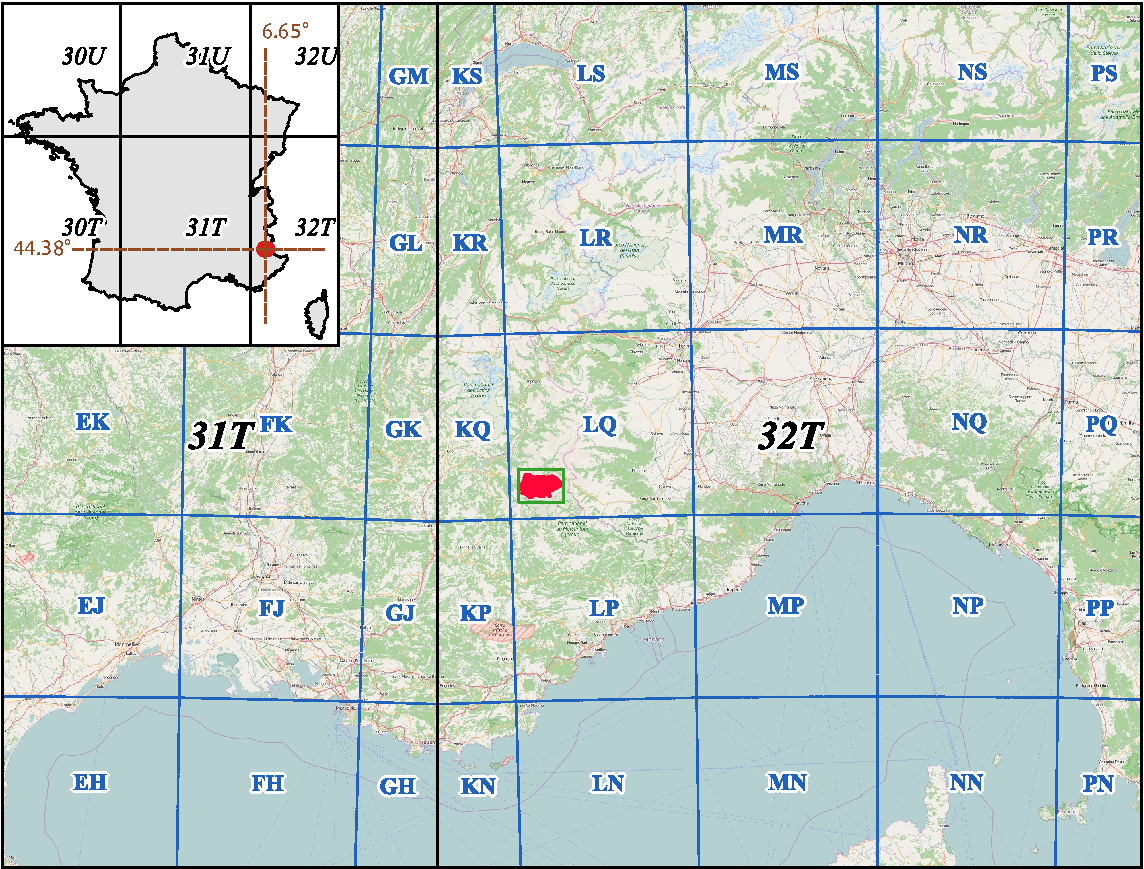
\includegraphics[width=\linewidth]{exemple/barc.pdf}
\caption{Zone d'étude de Barcelonnette représenté en rouge. Le rectangle représenté en vert et qui entoure Barcelonnette a pour coordonnées (longitude, latitude), \{(6.55, 44.31); (6.55, 44.47); (6.86, 44.47); (6.86, 44.31)\}. Ce rectangle est utilisé dans la requête OpenSearch afin de ne récupérer que les produits de l'archive qui intersectent ce rectangle. On peut également voir que la zone d'étude de Barcelonnette n'est située que sur la zone 32TLQ du système MGRS.}\label{fig:barc}
\end{figure}

\end{document}